\documentclass{article}
\usepackage[utf8]{inputenc}
\usepackage[backend=biber]{biblatex}
\usepackage{amssymb}
\usepackage{amsmath}
\usepackage{dsfont}
\addbibresource{bib.bib}
\setlength{\parindent}{0em}
\bibliography{bib}
\setlength{\parskip}{6pt}
\usepackage[margin=1.0in]{geometry}
\usepackage{graphicx}
\usepackage{caption}
\usepackage{subcaption}
\usepackage{wrapfig}
\usepackage{url}

\title{Intro to deep learning with PyTorch}
\author{Miguel A. Saavedra-Ruiz}
\date{Abril 2020}
\linespread{1.0}

\nocite{*}


\begin{document}

\maketitle

\section{Introduction to Neural Networks}

Deep learning is everywhere, applications in games such as Go or jeopardy, detecting spam in emails, forecasting stock prices, recognizing images in a picture, and diagnosing illnesses sometimes with more precision than doctors are just few examples.

The heart of Deep learning are object called \textbf{neural networks}. Neural networks vaguely mimic the process of how the brain operates, with neurons that fire bits of information. The next image shows a neural network \ref{fig:f1}.

\begin{figure}[ht]
    \centering
    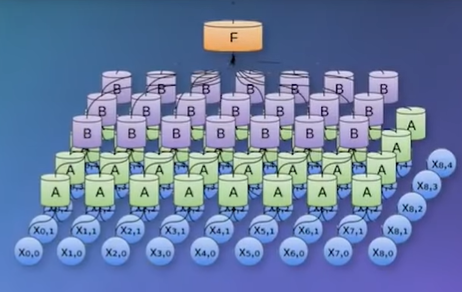
\includegraphics[width=0.35\textwidth,height=0.35\textheight,keepaspectratio]{images/nn.PNG}
    \captionsetup{justification=centering}
    \caption{A Neural network}
    \label{fig:f1}
\end{figure}

A neural network is a function approximator which is capable to split data. Given some data in the form of blue or red points, the neural network will look for the best line that separates the data \ref{fig:f2}..

\begin{figure}[ht]
    \centering
    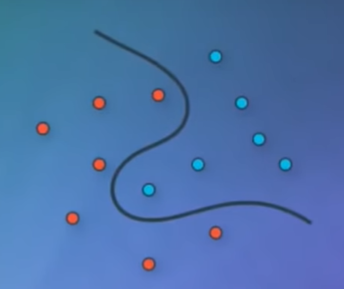
\includegraphics[width=0.2\textwidth,height=0.2\textheight,keepaspectratio]{images/data.PNG}
    \captionsetup{justification=centering}
    \caption{A Neural network splitting data}
    \label{fig:f2}
\end{figure}

The separation line is called a model and its job is to split the data. A model might not be perfect, but it most be as accurate as possible. Imagine the next example where we plot the acceptance rate of students based on their grades and test scores. The blue dots are accepted and red rejected. Furthermore, the line plotted is "the model" Fig. \ref{fig:f3}.

\begin{figure}[ht]
    \centering
    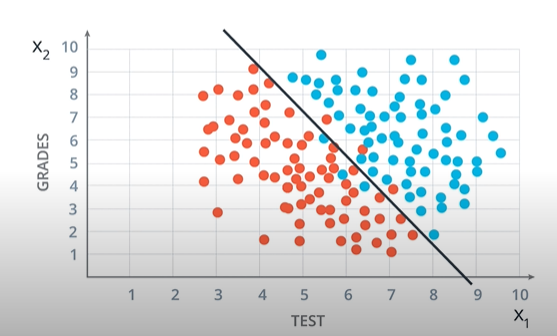
\includegraphics[width=0.5\textwidth,height=0.5\textheight,keepaspectratio]{images/example_1.PNG}
    \captionsetup{justification=centering}
    \caption{Neural network model}
    \label{fig:f3}
\end{figure}

Based on that, it is safe to predict that if a point is over the line the student gets accepted and if it's under the line then the student gets rejected.

Taking into account that Test is label as \(x_1\) and Grades as \(x_2\), the \textbf{boundary line} that separates the blue and the red points is going to have a linear equation. The equation of the one drawn above is describes in \eqref{eq:1}.

\begin{equation}
2 x_1 + x_2 - 18 = 0 \label{eq:1}
\end{equation}

The equation \eqref{eq:1} means that the method for accepting or rejecting students says the following: take this equation as our score where \(score =2.Test + Grades - 18\), if a student has \(score > 0\) the he gets accepted, otherwise he is rejected. This process is called a prediction. Additionally, by convention it is possible to say that if the score is 0, the student will get accepted although this won't matter much at the end. \textbf{The linear equation is out model}.

In the more general case, a boundary will be an equation of the following form \eqref{eq:2}.

\begin{equation}
wx_1+w_2x_2+b=0 \label{eq:2}
\end{equation}  

The last equation can be abbreviate in vector notation as \eqref{eq:3}.

\begin{equation}
wx+b=0 \label{eq:3}
\end{equation}  

Where w and x are vectors as shown below:

\[ w = (w_1, w_2)\]
\[ x = (x_1, x_2)\]

X can be refereed as the input, w as the weights and b as the bias. For a student coordinates \(x_1, x_2\), a label denoted as Y will be used as the value to predict. So if the student gets accepted, namely the point is blue,
then the label is \( y = 1\), And if the student gets rejected, namely the point is red and then the label is \( y = 0\)

The prediction made by our algorithm is going to be called \(\hat{y}\) and it will be what the algorithm predicts that the label will be \eqref{eq:4}. Where one means accepted and zero rejected.

\begin{equation}
\label{eq:4}
\hat{y} =
  \begin{cases}
    1, & \text{if } Wx + b \geq 0 \\
    0, & \text{if } Wx + b < 0 \\
  \end{cases}
\end{equation}  

So, to summarize, the points above the line have \( \hat{y} = 1\) and the points below the line have \( \hat{y} = 0\). And, the blue points have \( y = 1\) and the red points have \( y = 0\).

Subsequently, if we have more data columns so not just testing grades, but maybe something else like the ranking of the student in the class it will turn the problem into a three-dimensional space. The only difference now is that the problem won't be working in two dimensions but three. So now, the three axis are: \(x_1\) for the test, \(x_2\) for the grades and \(x_3\) for the class ranking. The data will looks like Fig. \ref{fig:f4}.

\begin{figure}[ht]
    \centering
    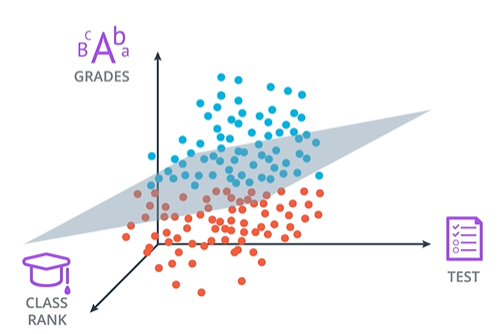
\includegraphics[width=0.5\textwidth,height=0.5\textheight,keepaspectratio]{images/example_2.PNG}
    \captionsetup{justification=centering}
    \caption{3D data example}
    \label{fig:f4}
\end{figure}

The equation won't be a line in two dimension, but a plane in three dimensions with a similar equation as before. Now, the equation would be \eqref{eq:5} which will separate this space into two regions.

\begin{equation}
w_1x_1 + w_2x_2 + w_3x_3 + b = 0, \label{eq:5}
\end{equation}  

This equation \eqref{eq:5} can still be abbreviated by \eqref{eq:3} (\(wx+b=0\)) except our vectors will now have three entries instead of two. The prediction will be the same as described by \eqref{eq:4}.

If we have many columns like say n of them as shown in Fig. \ref{fig:f5}, the data just leaps in n-dimensional space. Here the points are just things with n coordinates called \(x_1, x_2, x_3, \dots, x_n  \) with the labels being \(y\).

\begin{figure}[ht]
    \centering
    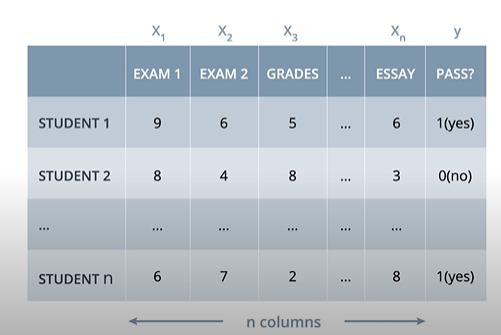
\includegraphics[width=0.5\textwidth,height=0.5\textheight,keepaspectratio]{images/multiple_dimension.PNG}
    \captionsetup{justification=centering}
    \caption{Multi-dimensional data}
    \label{fig:f5}
\end{figure}

Therefore, the boundaries just an \(n-1\) dimensional hyperplane, and the equation of this \(n-1\) dimensional hyperplane is going to be the one shown in \eqref{eq:6} or the abbreviated form shown in \eqref{eq:3} and the predictions still being the same as shown by equation \eqref{eq:4}.

\begin{equation}
w_1x_1 + w_2x_2 + \dots + w_n x_n + b = zero, \label{eq:6}
\end{equation}  

e.g Given the table in the Fig. \ref{fig:f5}, the dimensions for input features (x), the weights (W), and the bias (b) to satisfy (Wx + b) would be \( W(1xn), x(nx1) \text{and} b(1x1)\) for a single student.

Now it is time to introduce the notion of a \textbf{Perceptron}, which is the building block of neural networks. It is possible to show an example based on Fig. \ref{fig:f3}, where it is possible to encode the previous equations into a small graph. Let's fit The data and boundary line inside a node. Add small nodes for the inputs which in this case, they are the test and grades. The Fig. \ref{fig:f6} presents the mention before, with a specific value of test and grades. The Perceptron checks if the point is in the positive or negative area. If the point is in the positive area, then it returns a yes, otherwise a no.

\begin{figure}[ht]
    \centering
    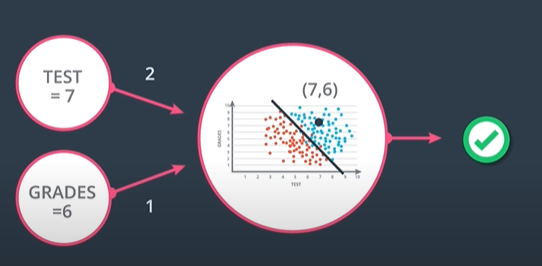
\includegraphics[width=0.5\textwidth,height=0.5\textheight,keepaspectratio]{images/perceptron_1.PNG}
    \captionsetup{justification=centering}
    \caption{Perceptron example with student admission}
    \label{fig:f6}
\end{figure}

Recall that the prediction consists of accepting the student based on \(score =2.Test + Grades - 18\), if the \( score \geq 0\) he gets accepted, and rejecting them if the \(score < 0\)

The weights \(2\), \(1\) and \(-18\) are what define the linear equation, and so they are used as labels in the graph Fig. \ref{fig:f6}. Another way to graph this node is to consider the bias as part of the input.

Since \(w_1\) gets multiplied by \(x_1\) and \(w_2\) by \(x_2\), it's natural to think that \(b\) gets multiplied by a one. So the bias will have the B labeling and and edge coming from a one. Then what the node does is it multiplies the values coming from the incoming nodes by the values and the corresponding edges. Then it adds them and finally, it checks if the result is greater than or equal to zero. If it is, then the node returns a yes or a value of one, and if it isn't then the node returns a no or a value of zero as shown in Fig. \ref{fig:f7}.

\begin{figure}[ht]
    \centering
    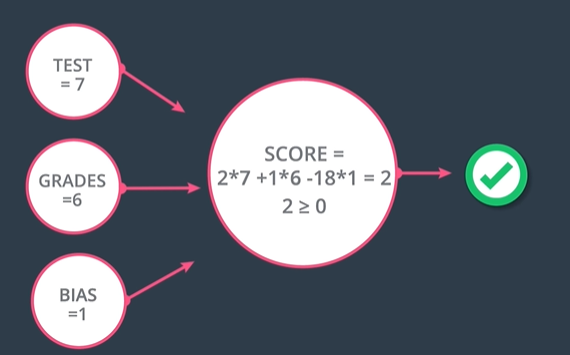
\includegraphics[width=0.45\textwidth,height=0.45\textheight,keepaspectratio]{images/perceptron_2.PNG}
    \captionsetup{justification=centering}
    \caption{Perceptron with weights and bias}
    \label{fig:f7}
\end{figure}

In the general case, a node looks like the one presented in Fig. \ref{fig:f8}.The node has inputs coming in with values \(x_1\) up to \(x_n\) and one (for the bias), and edges with weights \(w_1\) up to \(w_n\), and \(b\) corresponding to the bias unit. Then the node calculates the linear equation \eqref{eq:3}, which is this case is \(\sum_{i=1}^n w_i x_i + B\). This node then checks if the value is zero or bigger, and if it is, then the node returns a value of one for yes and if not, then it returns a value of zero for no. 

\[wx+b = \sum_{i=1}^n w_i x_i + b\]

\begin{figure}[ht]
    \centering
    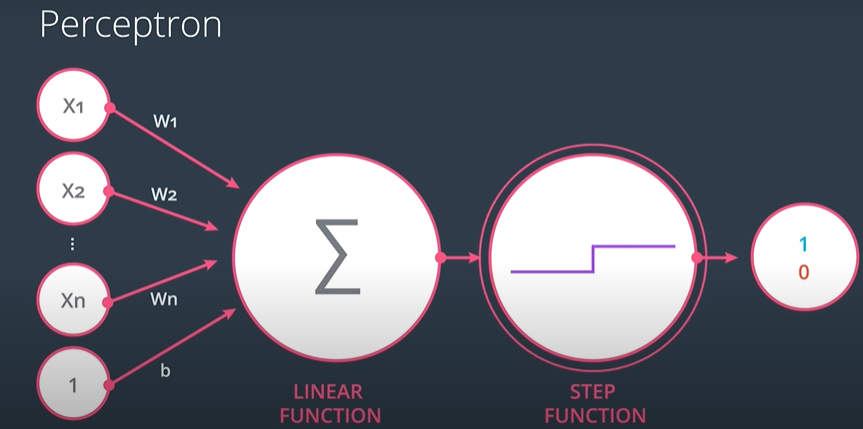
\includegraphics[width=0.5\textwidth,height=0.5\textheight,keepaspectratio]{images/general_perceptron.PNG}
    \captionsetup{justification=centering}
    \caption{General Perceptron}
    \label{fig:8}
\end{figure}

In the last Figure, an implicit function is being used, this is called a step function. What the step function does is it returns a one if the input is positive or zero if the input is negative Fig. \ref{fig:f9}.

\begin{figure}[ht]
    \centering
    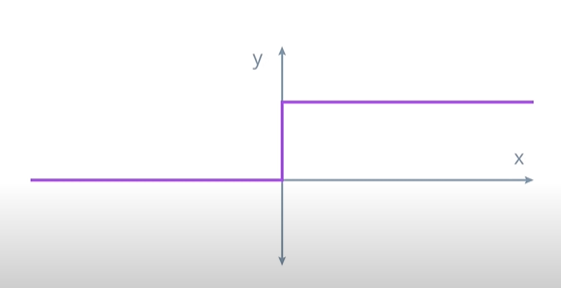
\includegraphics[width=0.4\textwidth,height=0.4\textheight,keepaspectratio]{images/step.PNG}
    \captionsetup{justification=centering}
    \caption{Step function}
    \label{fig:f9}
\end{figure}

\[
y =
  \begin{cases}
    1, & \text{if } x \geq 0 \\
    0, & \text{if } x < 0 \\
  \end{cases}
\]

In reality, the perceptron can be seen as a combination of nodes, where the first node calculates a linear equation based on the inputs and weights. The second node applies the step function to the result, giving the final outcome of the perceptron Fig. \ref{fig:f10}. The \(\sum\) represents a linear function in the first node and the drawing represents a step function in the second node. Nevertheless, we can use different step functions or generally, activation functions in this node.

\begin{figure}[ht]
    \centering
    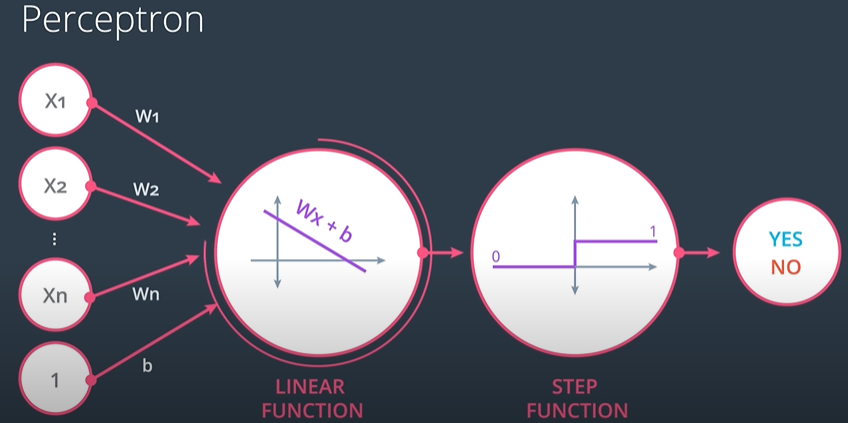
\includegraphics[width=0.5\textwidth,height=0.5\textheight,keepaspectratio]{images/simple_perceptron.PNG}
    \captionsetup{justification=centering}
    \caption{The simple perceptron}
    \label{fig:f10}
\end{figure}

The name "neural network" comes from the fact that perceptrons look like neurons in the brain. In the Fig. \ref{fig:f11} can be seen a perceptron in the Left with four inputs, these inputs are the dendrites in a Neuron and they receive nervous impulses. Similarly, the computation is made in the node of the perceptron or nucleus. Finally, the perceptron outputs the final result as a neuron does through its axon, which is the mechanism a neuron use to outputs nervous impulses. \textbf{The neural networks mimic the concept of neuron and brain} by taking the output from one neuron and turning it into the input for another one.

\begin{figure}[ht]
    \centering
    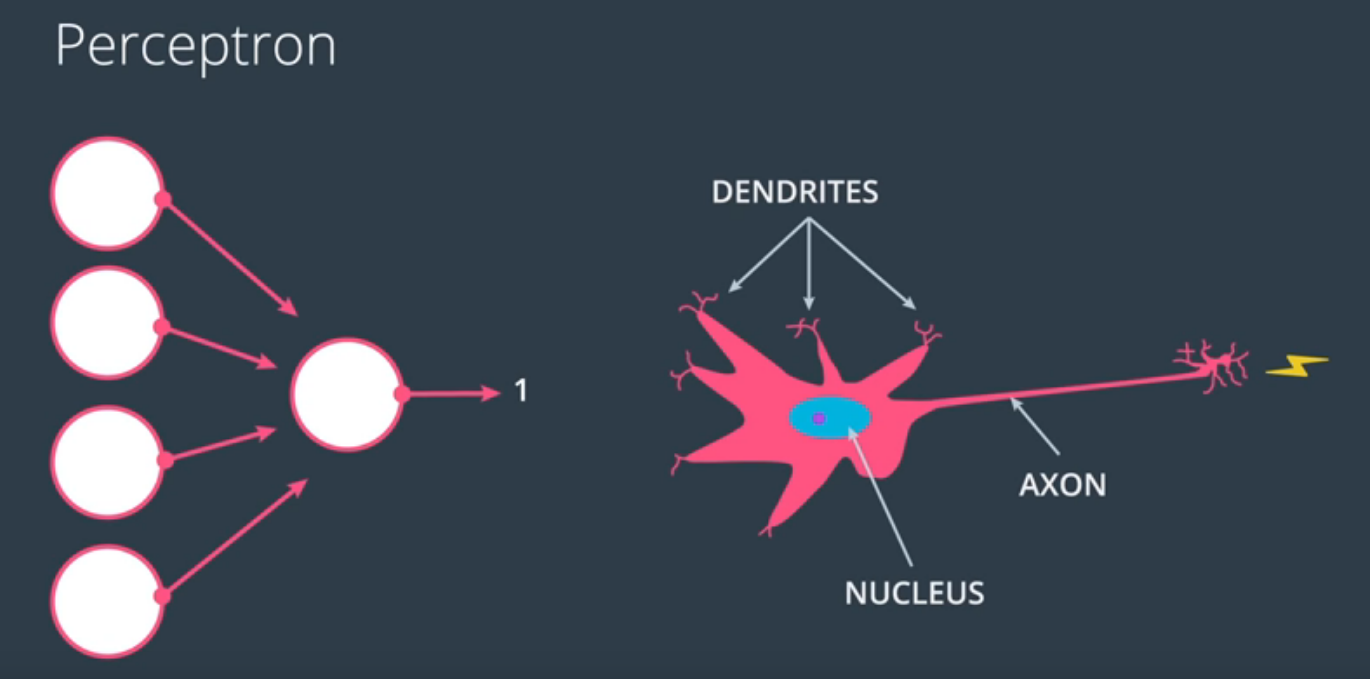
\includegraphics[width=0.5\textwidth,height=0.5\textheight,keepaspectratio]{images/perceotron_neuron.png}
    \captionsetup{justification=centering}
    \caption{The perceptron as a neuron}
    \label{fig:f11}
\end{figure}

Perceptrons can be used as logic operators (AND, OR, XOR). E.g the ND operator can be represented as a two inputs perceptron with 1 output, where the inputs can be 1 or 0 as well as the output. To recall the true table of the perceptron, it is presented in Fig. \ref{fig:f12}. The perceptron presented in the same figure shows how it splits the points with a boundary line, where the dots in the red area corresponds to a zero and the point in the blue area corresponds to a one. In the file called \textit{introduction/and\_perceptron.py} can be seen an example of this which use the general equation of a boundary \eqref{eq:2} (\(wx_1+w_2x_2+b=0\)). 

\begin{figure}[ht]
    \centering
    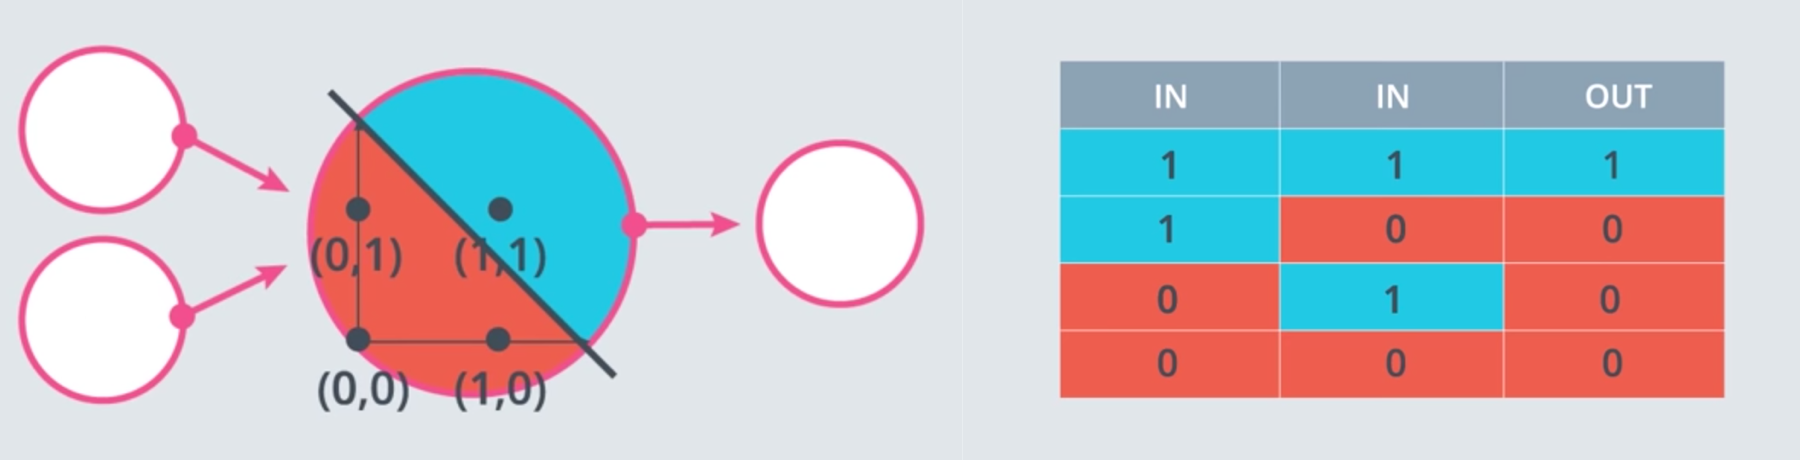
\includegraphics[width=0.5\textwidth,height=0.5\textheight,keepaspectratio]{images/and_table.png}
    \captionsetup{justification=centering}
    \caption{True table of the AND operator}
    \label{fig:f12}
\end{figure}

It is possible to represent logic operators as AND or OR with simple perceptrons, nevertheless, a problem arises when the problem has non-linear boundaries. 

To find the boundary line for a simple logic operator the process is really straightforward. Imagine a classification problem as shown by Fig. \ref{fig:f13}, the goal is to classify both the blue and red points correctly. However, there are one blue point and red point misclassified. To solve this, one logic approach would be to make the line closer to the misclassified points (located in the blue region) and hence change its label.

\begin{figure}[ht]
    \centering
    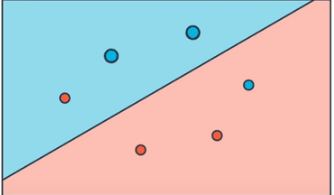
\includegraphics[width=0.25\textwidth,height=0.25\textheight,keepaspectratio]{images/split_data.png}
    \captionsetup{justification=centering}
    \caption{Splitting the data example}
    \label{fig:f13}
\end{figure}

Now imagine the line plotted in Fig. \ref{fig:f14}, where the line equation is given by \(3x_1+ 4x_2 - 10 = 0\) and out labels are: blue area if \(\hat{y} > 0\) or red area if \(\hat{y} < 0\). Suppose that the line has coordinates \((4,5)\), based on the approach described above, the point coordinates should be subtracted to the line equation as shown by the equation below, where \(x_1 = 4, x_2 = 5 \text{ and } b = 1\).

\[
\begin{bmatrix}  \text{new } w_1 \\
                 \text{new } w_2 \\
                \text{new } b \end{bmatrix} = \begin{bmatrix}
                                    3 - 4 \\
                                    4 - 5 \\
                                    -10 - 1
                                    \end{bmatrix} = \begin{bmatrix}
                                                    -1 \\
                                                    -1 \\
                                                    -11
                                                    \end{bmatrix}
\]

\begin{figure}[ht]
    \centering
    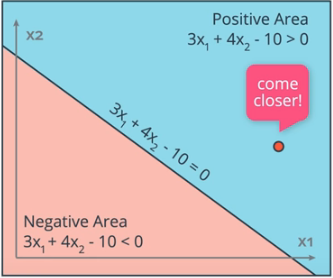
\includegraphics[width=0.25\textwidth,height=0.25\textheight,keepaspectratio]{images/moving_line.png}
    \captionsetup{justification=centering}
    \caption{Making the line closer example}
    \label{fig:f14}
\end{figure}

With the new parameters, the equation will be \(-1x_1+ 4-1x_2 - 11 = 0\). Nevertheless, this might be a very drastic change in the equation, leading to misclassification of other well-classified points. The idea is to make the line take small moves towards the misclassified point. To solve this, it is neccesary to take small steps towards the point, therefore, a new concept needs to be introduced. This concepts is called \(\alpha\) or \textbf{learning rate}. The learning rate is a small number between zero and one and its function is to minimize the change in the model equation by multiplying its value to the values of the point. E.g, using a learning rate of \(0.1\) and the same example as before, the result will be the shown in the equation and Fig. \ref{fig:f15}

\[
\begin{bmatrix}  \text{new } w_1 \\
                 \text{new } w_2 \\
                \text{new } b \end{bmatrix} = \begin{bmatrix}
                                    3 - 4*(0.1) \\
                                    4 - 5*(0.1) \\
                                    -10 - 1*(0.1)
                                    \end{bmatrix} = \begin{bmatrix}
                                                    2.6 \\
                                                    3.5 \\
                                                    -10.1
                                                    \end{bmatrix}
\]

\begin{figure}[ht]
    \centering
    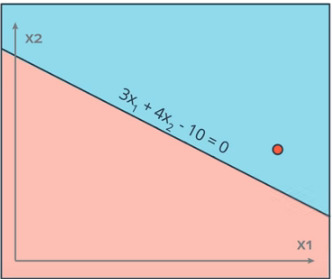
\includegraphics[width=0.25\textwidth,height=0.25\textheight,keepaspectratio]{images/new_line.png}
    \captionsetup{justification=centering}
    \caption{Moving the line closer to the point}
    \label{fig:f14}
\end{figure}

Similarly, if the misclassified point is located in the red area, instead of subtracting the point to the model equation it needs to be added. As a thumb rule, the \eqref{eq:7} shows the process of adding or substracting based on the point's location.

\begin{equation}
\label{eq:7}
  \begin{cases}
    Substract, & \text{if } \text{point is located in region } > 0 \\
    Add, & \text{if } \text{point is located in region } < 0 \\
  \end{cases}
\end{equation}  

Based on the technique given above, it is possible to determine the perceptron algorithm. This one is presented in the Fig. \ref{fig:f16} and shows and iterative process that tries to classify correctly all the misclassified points. The process works iteratively and can run until all the points are correctly classified or a minimum of misclassified points are obtained. A code example of this is given in \textit{introduction/perceptron\_algorithm.py}
  
\begin{figure}[ht]
    \centering
    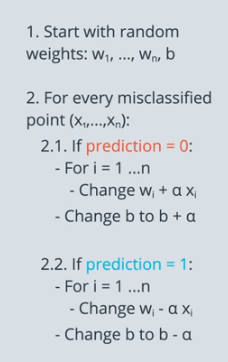
\includegraphics[width=0.2\textwidth,height=0.2\textheight,keepaspectratio]{images/perceotron_algorithm.png}
    \captionsetup{justification=centering}
    \caption{The perceptron Pseudocode}
    \label{fig:f16}
\end{figure}
  
Let's look more carefully at the model presented in Fig. \ref{fig:f3} for accepting and rejecting students. Imagine that the student four got nine in the test but only one on the grades. According to the model this student gets accepted since it's placed in the positive region of this line. Nevertheless, this is not accurate. A more precise model is presented in Fig. \ref{fig:f7}, however, this is non-linear separable. To create an accurate model a different boundary should be used, two lines, a circle or a polynomial function are just few examples of this. Unfortunately, \textbf{the perceptron algorithm won't work well for non-linear problems}. Therefore, something more complex needs to be applied to redefine the simple perceptron algorithm for a line in a way that it'll generalize to other types of curves.

\begin{figure}[ht]
    \centering
    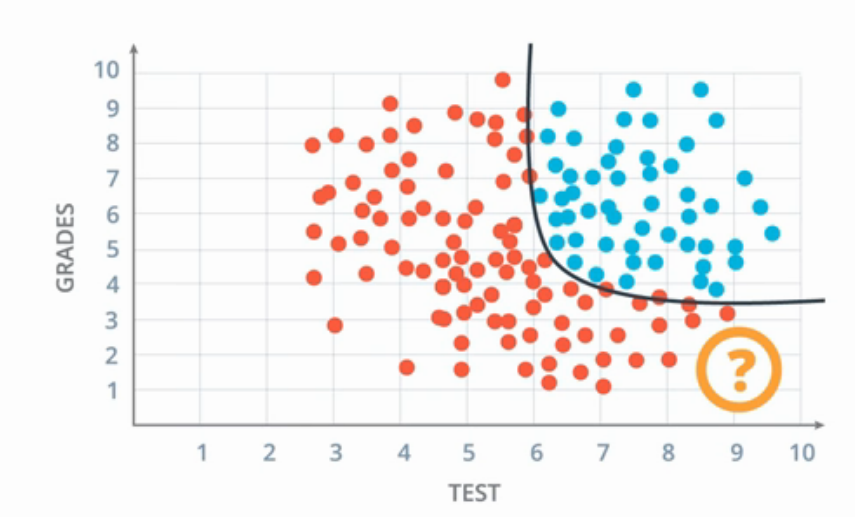
\includegraphics[width=0.35\textwidth,height=0.35\textheight,keepaspectratio]{images/non_linear.png}
    \captionsetup{justification=centering}
    \caption{Non-linear area}
    \label{fig:f17}
\end{figure}

To tackle Deep learning problems, it is necessary to introduce the concept of \textbf{Error function}. This is simply something that tells how far is the current model from the solution. An example of a simple error function used in the last example would be a function that tells how far is a point from its good classification region (distance).

\textbf{Gradient descent} is a method to reduce the error of a problem and find the global optimum using known metrics. This algorithm calculates the error and then takes a step towards the direction that minimizes the error in a problem. As an example for the Fig. \ref{fig:f13} it is possible to construct an error function which consists of the sum of the distance of the points to the boundary lines, where the misclassified points have a big penalty while the well classifies have a low penalty. This function can be used to guide the boundary line towards a direction that minimizes the error and thus, find the optimal model to solve the problem. \textbf{Note:} the error function should be differentiable and continuous. 

Recall that a discrete prediction might be something like a 1 or zero, whereas a continuous prediction would be a number, normally between zero and one. As an example, see the  Fig. \ref{fig:f18} where we have students with discrete predictions (left) and continuous predictions(right). In the discrete plot, the algorithm will tell if a student is accepted (1 - blue) or rejected (0 - red). In the continuous plot, the farther the point is from the black line, the more drastic these probabilities are. Points that are well into the blue area get very high probabilities And points that are well into the red region are given very low probabilities. The points over the line are all given a 50\% probability. The probability is a function of the distance from the line.

\begin{figure}[ht]
    \centering
    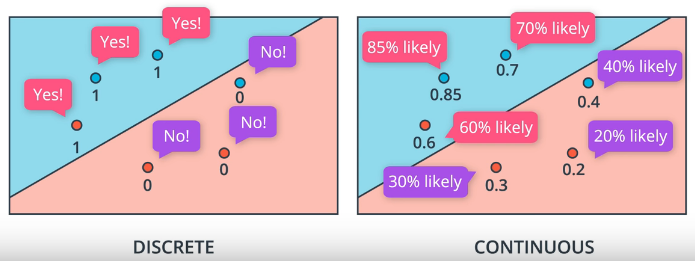
\includegraphics[width=0.5\textwidth,height=0.5\textheight,keepaspectratio]{images/discrete_continuous.png}
    \captionsetup{justification=centering}
    \caption{Discrete and continuous predictions}
    \label{fig:f18}
\end{figure}

To change from discrete to continuous predictions it is necessary to use a \textbf{Sigmoid function} (Fig. \ref{fig:f19}) instead of a unitary step as the activation function. This activation will guarantee a continuous functions instead of a discrete one, allowing the usage of gradient descent techniques. The equation of the Sigmoid function is given in the Equation \eqref{eq:8}. Before the model consisted of a line with a positive region and a negative region. With the Sigmoid function now it consists of an entire probability space for each point in the plane.

\begin{figure}[ht]
    \centering
    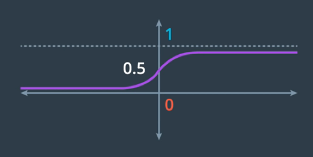
\includegraphics[width=0.35\textwidth,height=0.35\textheight,keepaspectratio]{images/sigmoid.png}
    \captionsetup{justification=centering}
    \caption{Sigmoid function}
    \label{fig:f19}
\end{figure}

\begin{equation}
\label{eq:8}
\sigma(x) = \frac{1}{1 - e^{-x}} 
\end{equation}  

Using the Sigmoid function as the activation function to predict \(\hat{y}\), the output of the perceptron will be as follows Eq. \eqref{eq:9}. The simple perceptron seen in Fig. \ref{fig:f8} with a step function can be modified as shown by Fig. \ref{fig:f20} to work with a Sigmoid function as the activation function.  Before it used to say the student got accepted or not, with the Sigmoid function it says the probability of the student got accepted is this much.

\begin{equation}
\label{eq:9}
\hat{y} = \sigma(Wx + b)
\end{equation} 

\begin{figure}[ht]
    \centering
    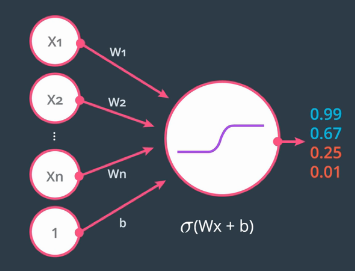
\includegraphics[width=0.30\textwidth,height=0.30\textheight,keepaspectratio]{images/perceptron_sigmoid.png}
    \captionsetup{justification=centering}
    \caption{Simple perceptron with a sigmoid activation function}
    \label{fig:f20}
\end{figure}
%\printbibliography

\end{document}
